\chapter{Scramble architecture}
\label{ch:Scramble architecture}

Scramble is a tool to realize scalability with hierarchical orchestration. While the higher level orchestrator (Parent MANO) still controls the life-cycle of the deployed network services, scramble acts as a bridge between parent MANO and lower level orchestrator (child MANO) thus allowing interconnection between differnt MANO's to provide end-to-end service.  
 
\section{Architecture}
\paragraph{}
The services of scramble resides as a plugin within MANO frameworks such as SOTANA/Pishahang and Open Source MANO (OSM) and allows such MANO frameworks to be added as child MANO. Any request received by Parent MANO for service instantiation is passed on to scramble plugin which based on monitoring parameters collected from child MANO's decides where the service has to be instantiated.

\paragraph{}
Each child MANO's in-turn contains scramble plugin which allows multiple other MANO's to be added as a child hence achieving hierarchical orchestration.

\paragraph{}

Scramble is composed of three main services.
\begin{itemize}
	\item Translator
	\item Splitter
	\item Wrapper(adopter)
	\end{itemize} 
Each of these services are further explained in-detail in sections \ref{ch:Scramble wrapper architecture}, \ref{ch:Scramble splitter architecture}, \ref{ch:PMW} accordingly.

\begin{figure} [h]
	\centering
	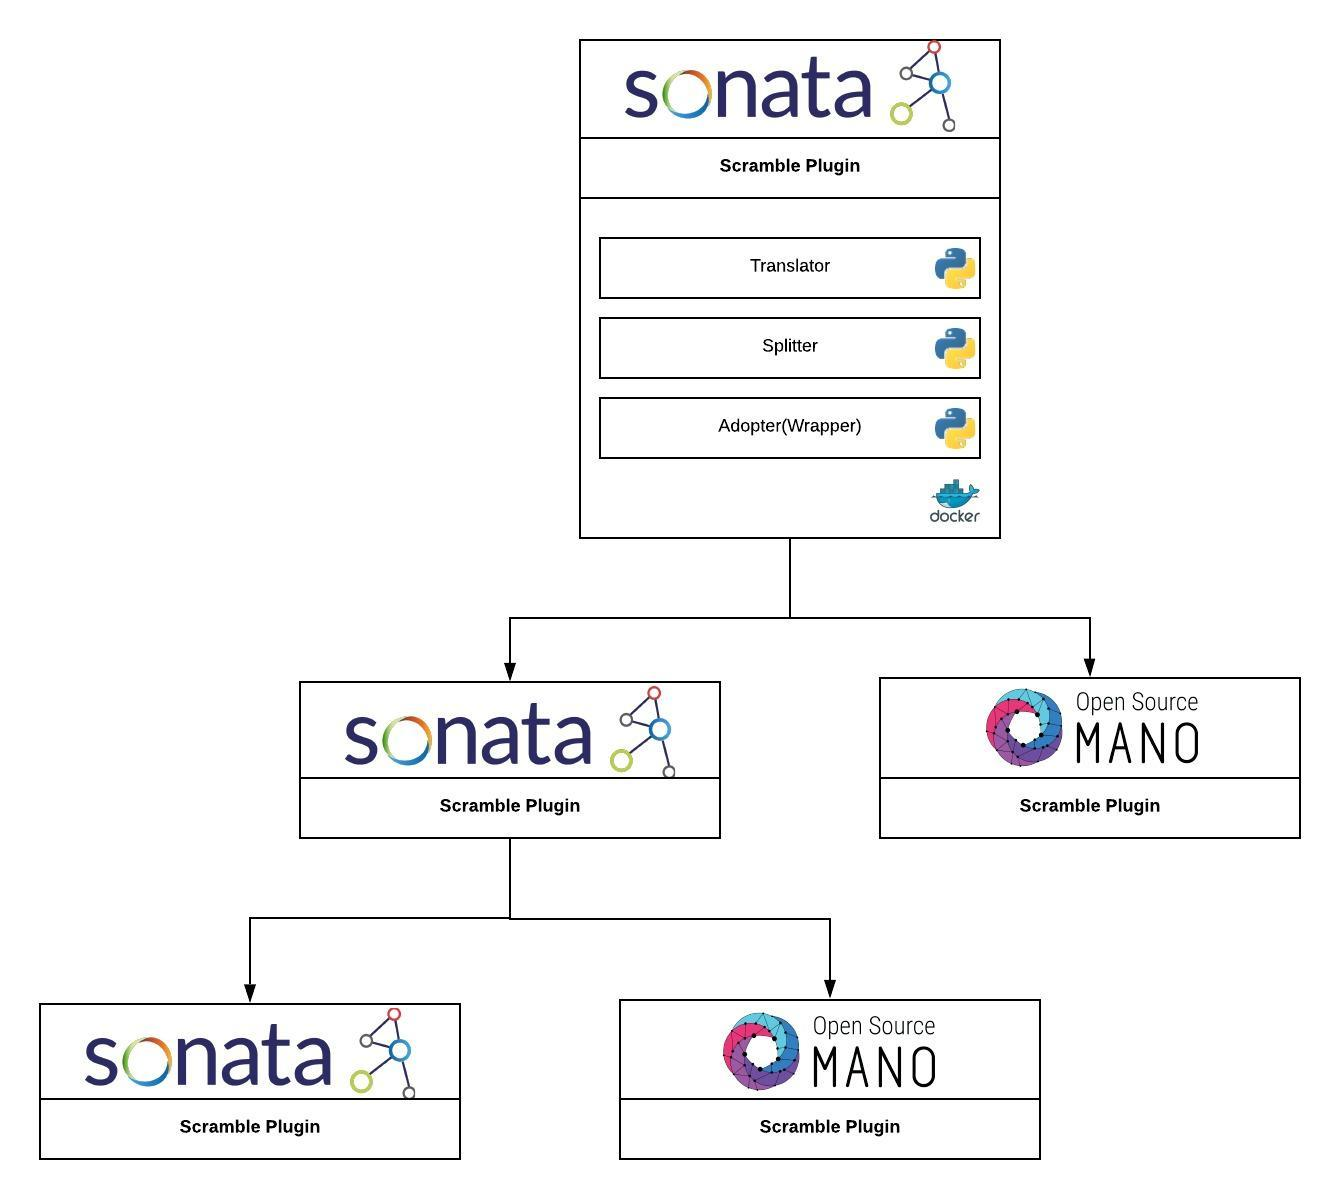
\includegraphics[width=1\linewidth]{figures/scramblearch}
	\caption{Scramble Architecture}
	\label{fig:scramblearch}
\end{figure}
